\section{Implementation}\label{techUse}
There are two categories of components : the client and the server, for which the followings parts presents various functionnalities.
\begin{figure}[!h]
			\centering
			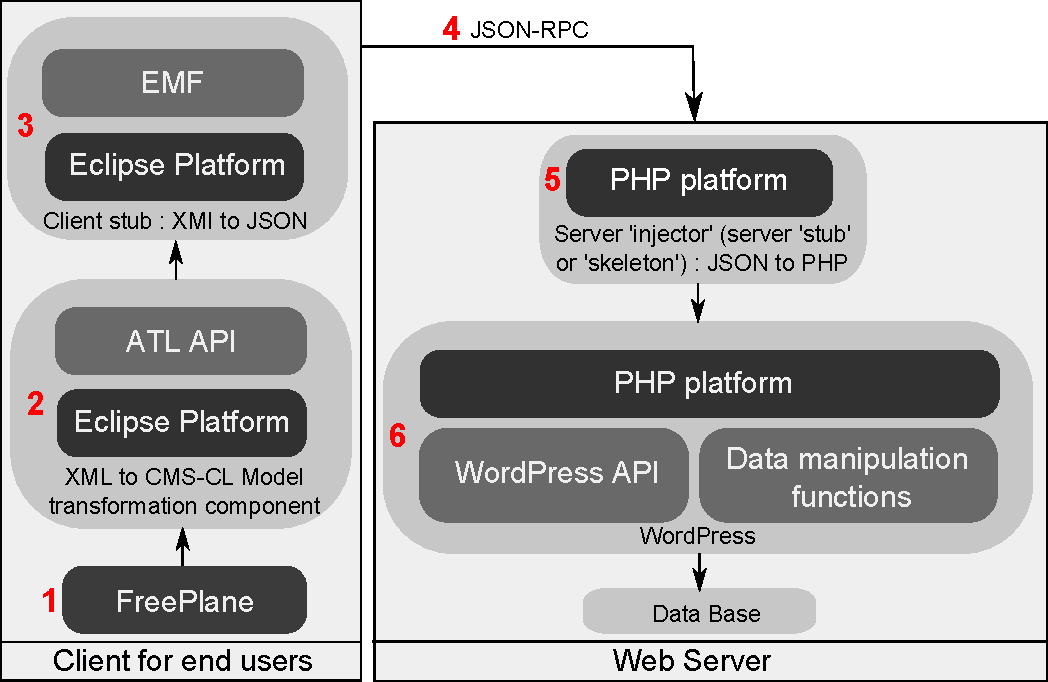
\includegraphics[width=0.85\textwidth]{../resources/pdf/final_ClientServer_numbered.pdf}
			\caption{Client-server complete process}
			\label{finalClientServer}
\end{figure}

	\subsection{Client part}	
		\vspace{0.15em}
		\noindent\textbf{Mind mapping (\textcolor{red}{1}).} To manipulate concepts with the mind mapping, the end-users use the Freeplane GUI and one of its output format which is the XML. With Freeplane, the users create a mind map (see section \ref{CMS-CL}, paragraph \ref{concreteSyntax}) of the different elements they want to manage for their web site.
%			\begin{figure}[!h]
%				\centering
%				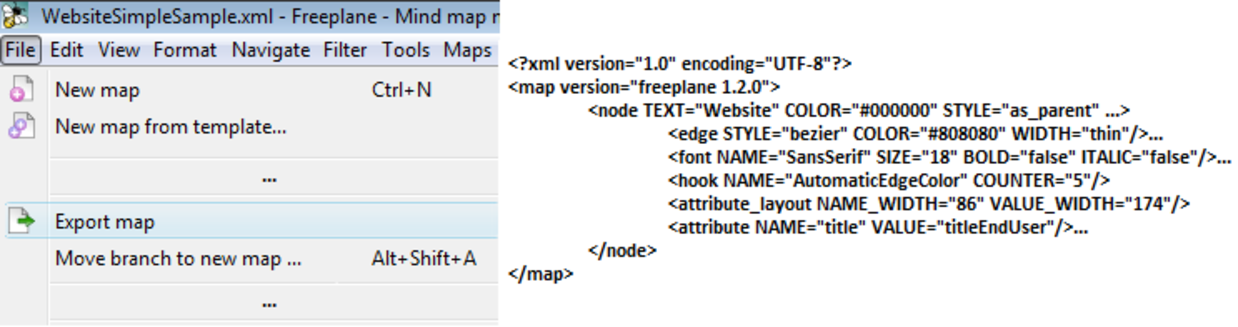
\includegraphics[width=\textwidth]{../resources/pdf/freePlaneUI_XML.pdf}
%				\caption{FreePlane : Export of the mind map and its xml output sample}
%				\label{freePlaneUI}
%			\end{figure}
			Then, via the export menu, they get a file representing this mind map, in an XML format\footnote{Extensbile Markup Language}\cite{xmlPresent}. There are other formats proposed (svg, mwiki, html, jpg, odt), but XML has some advantages that the other ones do not have : information structure is easily discerned by both humans and computers and it is application-independent.			
			
		\vspace{0.15em}
		\noindent\textbf{Transformation to CMS-CL model (\textcolor{red}{2}).} The XML representation must be now transformed in a CMS-CL model. For this, ATL\footnote{AtlanMod Transformation Language} is used : it is a model transformation language an Eclipse plugin. The output CMS-CL model is used by a third client component whose the description is done bellow.
		
		\vspace{0.15em}
		\noindent\textbf{Client 'stub' (\textcolor{red}{3}).} This component is called a 'stub' because it allows to have the same data format between the client and the server for the data interchange : the client parse (it is called 'marshalling') the data in JSON. So, the CMS-CL model is transformed to this common data interchange format by using the EMF\footnote{Eclipse Modeling Framework} \cite{emfPresent} on Eclipse.		
		The choosen format was JSON (see the listing\ref{jsonOutput} example) because it is specialized for data interchange, which is the case between the client and the server. It would be possible to have a direct transformation to this format (XML-to-JSON), but there are four reasons we choose to do this in two steps ('XML-to-CMS-CL' and 'CMS-CL-to-JSON') : \textit{Maintenability} (only the 'CMS-CL-to-JSON' transformation would be changed on a data interchange format modification),  \textit{Productivity} (if it is easier to maintain, it is also a gain of time), \textit{Readability} (with a one step process, we would have more complex metamodels, which is less readable), and \textit{Reusability} (each transformations could be usable by other components).
			\lstset{
  								caption=Web site elements in JSON, 
  								label=jsonOutput,
 								basicstyle=\scriptsize,
  								xleftmargin=.110\columnwidth , xrightmargin=.110\columnwidth
						}
			\begin{lstlisting}
{"website" : { "adminUser": { "idUser":"userOne", ... } }, ... }			
			\end{lstlisting}
	
	\subsection{Communication between Server and Client (\textcolor{red}{4})}
	The communication between the client and the server parts use the JSON-RPC\cite{jsonRpc} protocol : it uses the RPC protocol to call server methods, and the requests are in the JSON format.			
	\subsection{Server part}
		\textbf{Injector (server 'stub' or 'skeleton') (\textcolor{red}{5}).} This injector -also called the server 'stub' or 'skeleton'- consists to do the inverse of the 'stub' on the client side, i.e. to unparse the parameters (also called 'unmarshalling') and call its local WordPress functions with the parameters.
					
		\vspace{0.15em}
		\noindent\textbf{API and Data manipulations functions (\textcolor{red}{6}).} The functions called by the injector are divided in two types : those available in the WordPress API and those which are not remotely callable. But all of them send data to the data base, allowing a website update.	
	
	